\newpage\pagestyle{main}

\chapter{Sviluppo del Sistema: Distribuzione e Sincronizzazione}\label{chap:third}

\inlineminitoc

% ─────────────────────────────────────────────────────────────────────────────
\section{Logica dello Sharding: Gestione dinamica dei dati}

In un ecosistema di Intelligenza Artificiale Conversazionale, la velocità di risposta
è un fattore critico per l'accettazione da parte dell'utente \cite{latency_eca}.
La percezione di naturalezza in un dialogo con un agente virtuale dipende in misura
significativa dalla latenza: risposte che arrivano dopo più di qualche secondo
interrompono il flusso conversazionale e degradano l'esperienza utente, indipendentemente
dalla qualità del contenuto della risposta stessa. In contesti come quello medico,
dove l'utente può trovarsi in uno stato di preoccupazione o urgenza, questo aspetto
diventa ancora più rilevante.

Il problema fondamentale è un \textbf{trade-off} tra completezza e velocità. Da un
lato, la base di conoscenza deve essere completa e aggiornata, il che richiede di
mantenerla su un server centrale accessibile da qualsiasi istanza del sistema. Dall'altro,
ogni interrogazione a un database remoto introduce una latenza di rete che, sommata
agli altri tempi di elaborazione del sistema, può superare facilmente la soglia di
tollerabilità. Il caricamento dell'intera base di conoscenza in memoria locale
sarebbe la soluzione ideale in termini di velocità, ma è spesso impraticabile: un
database medico realistico può contenere milioni di nodi, e trasferire e mantenere
sincronizzata una copia locale di queste dimensioni richiederebbe risorse computazionali
e di storage non disponibili su hardware consumer.

Per risolvere questo trade-off, il sistema adotta una logica di \textbf{sharding}
basata sulla distinzione tra due livelli di memorizzazione con caratteristiche
complementari:

\begin{itemize}
    \item \textbf{Remote Knowledge Base}: Un repository completo e persistente,
          ospitato su un server centrale, che contiene la totalità delle informazioni
          disponibili. È la fonte di verità del sistema: aggiornata centralmente, sempre
          coerente, ma soggetta a latenza di rete variabile a ogni interrogazione.

    \item \textbf{Local Shard}: Una memoria ad alte prestazioni, situata sullo
          stesso host che esegue il backend Python e i modelli Ollama, che contiene
          solo il sottoinsieme di dati rilevante per la sessione conversazionale corrente.
          Essendo locale, le sue interrogazioni avvengono senza latenza di rete, con
          tempi di risposta paragonabili a quelli di un accesso in memoria.
\end{itemize}

Questa architettura si ispira ai concetti di \textit{Caching} e \textit{Data Sharding}
descritti da Kleppmann \cite{kleppmann2017}, adattandoli però alle necessità specifiche
dei database a grafo, dove la \textbf{vicinanza topologica} tra i nodi è altrettanto
importante della vicinanza temporale degli accessi. Nei database relazionali o
documentali tradizionali, una strategia di caching basata sulle singole righe o
documenti più acceduti è sufficiente. In un database a grafo, invece, è fondamentale
portare in cache non solo il nodo richiesto, ma anche i suoi vicini strutturali —
i paragrafi adiacenti nel documento, il nodo documento genitore — perché è la
navigazione di questi collegamenti, e non il nodo isolato, a fornire il contesto
ricco necessario all'LLM.

\begin{figure}[htbp]
    \centering
    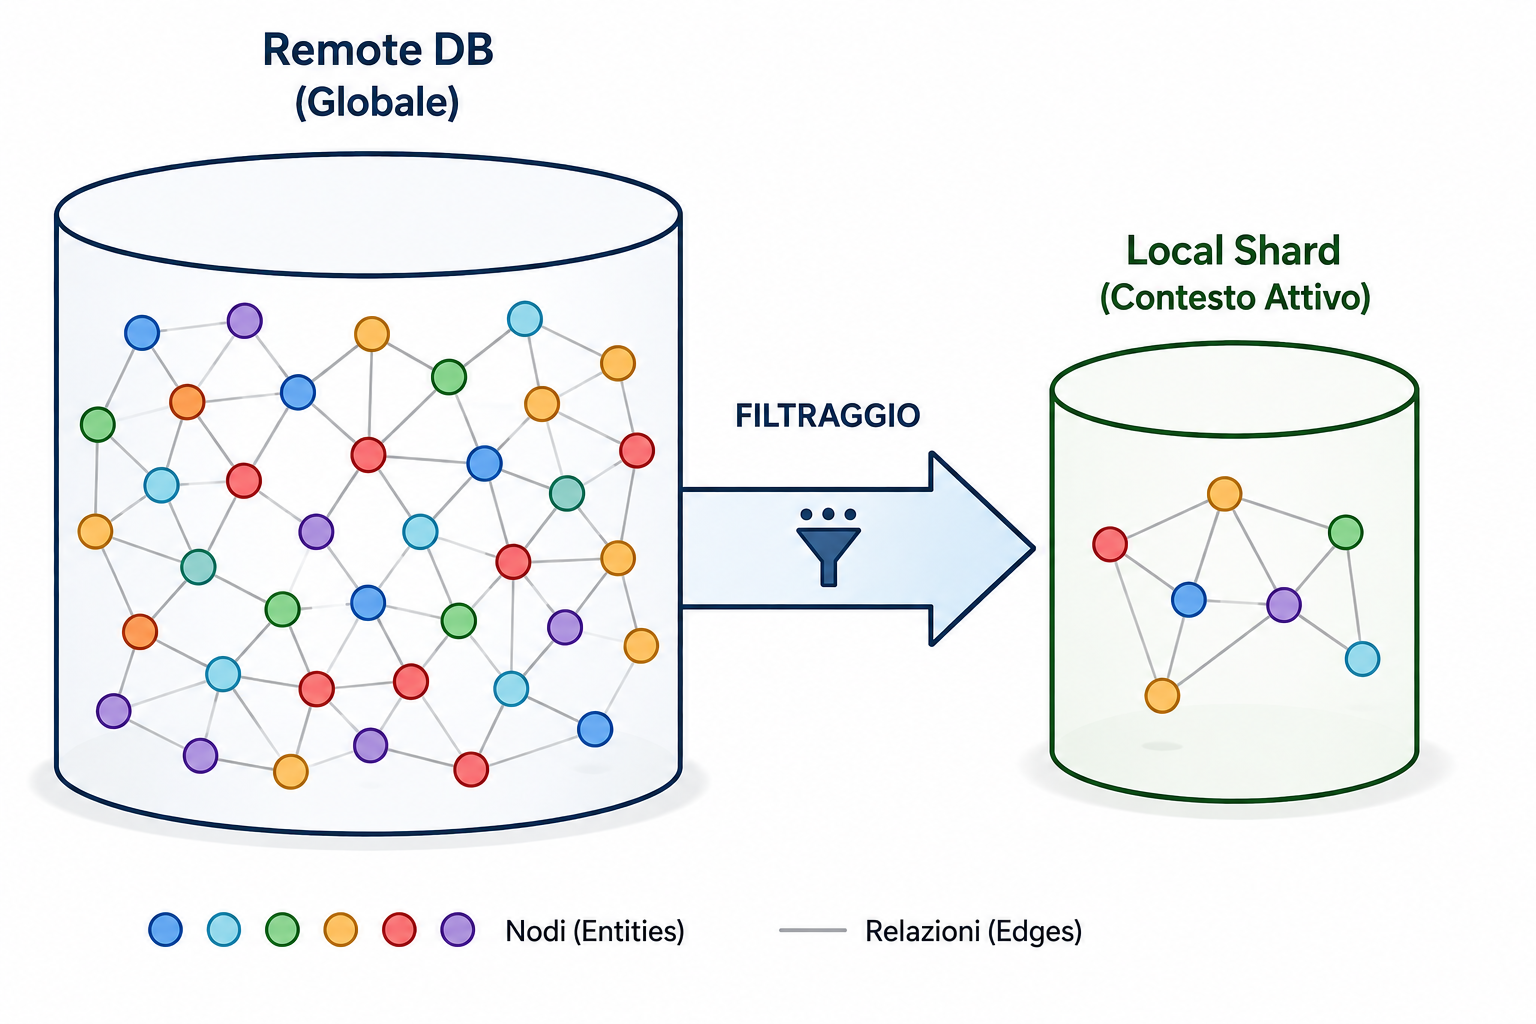
\includegraphics[width=0.8\textwidth]{_figures/sharding_levels.png}
    \caption{Rappresentazione dei due livelli di memorizzazione: Remote DB (Globale)
        e Local Shard (Contesto Attivo). Il filtraggio selettivo garantisce che solo i
        dati ``caldi'' — quelli acceduti frequentemente nella sessione corrente — vengano
        mantenuti nello Shard locale, mentre il Remote rimane la fonte di verità completa.}
    \label{fig:sharding_levels}
\end{figure}

% ─────────────────────────────────────────────────────────────────────────────
\section{Il ciclo di vita della query distribuita}

L'interazione con il sistema non è una semplice operazione di lettura su un singolo
database, ma un \textbf{processo ciclico} coordinato dall'orchestratore Python tramite LangGraph. Ogni volta che l'agente necessita di recuperare informazioni dalla Knowledge Base, viene eseguita una sequenza di operazioni che attraversa entrambi i livelli dell'architettura distribuita: il Remote, per la ricerca vettoriale sull'indice completo, e lo Shard locale, per la sincronizzazione, la manutenzione della cache e il recupero finale del contesto da fornire all'LLM.
Il cuore tecnologico di questo processo è l'integrazione tra la ricerca vettoriale
e la manipolazione del grafo in un'unica transazione atomica, realizzata sfruttando
le funzionalità avanzate di Neo4j per la gestione di database compositi distribuiti.

% ─────────────────────────────────────────────────────────────────────────────
\subsection{L'uso delle Call Subqueries}

Per implementare questa logica complessa in Neo4j mantenendo al contempo l'atomicità
dell'operazione, si è fatto ricorso alle \textbf{Call Subqueries} \cite{neo4j_subqueries}.
Le Call Subqueries permettono di eseguire blocchi di logica Cypher separati all'interno
di una query principale, specificando per ciascuno su quale database del cluster deve
essere eseguito tramite la clausola \texttt{USE}. Questa funzionalità è la chiave
che rende possibile coordinare operazioni su database fisicamente distinti — il Remote
e lo Shard — nell'ambito di un'unica chiamata dal layer applicativo Python.

La scelta di accentrare tutta la logica in un'unica macro-query, anziché distribuirla
su più chiamate separate dal codice Python, è motivata da ragioni sia di prestazioni
sia di correttezza. Dal punto di vista delle prestazioni, ogni chiamata da Python al
database comporta un overhead di serializzazione, trasmissione di rete e
deserializzazione. Ridurre il numero di round-trip significa ridurre proporzionalmente
questo overhead: con la macro-query, Python effettua una sola chiamata e riceve un
solo risultato, indipendentemente dalla complessità delle operazioni eseguite
internamente. Senza questa funzionalità, il sistema dovrebbe scaricare i dati in
Python, elaborarli in memoria e reinviarli al database locale, potenzialmente
raddoppiando i tempi di comunicazione.

Dal punto di vista della correttezza, avere tutta la logica in una singola transazione
garantisce che le operazioni di lettura dal Remote e di scrittura sullo Shard siano
coerenti tra loro: non è possibile che una lettura riesca e la scrittura successiva
fallisca lasciando lo Shard in uno stato parziale, perché entrambe le operazioni
fanno parte della stessa unità di lavoro transazionale. Con le subqueries, lo
spostamento dei dati tra Remote e Shard avviene in modo quasi trasparente per
l'applicazione Python, che vede semplicemente una chiamata con un parametro
(il vettore della query) e un risultato (i paragrafi contestuali da fornire all'LLM).

Un ulteriore vantaggio delle Call Subqueries è la possibilità di implementare
\textbf{logica condizionale} tramite la sintassi \texttt{WHEN...THEN}. Questa funzionalità è
fondamentale per la logica di \textit{upsert}: in base al fatto che un nodo sia
già presente o meno nello Shard, il sistema esegue azioni diverse — creazione ex
novo o semplice aggiornamento dei metadati — senza dover uscire dalla query per
effettuare questo controllo a livello applicativo.

\newpage

% ─────────────────────────────────────────────────────────────────────────────
\section{Implementazione della logica di sincronizzazione}

Di seguito viene analizzata nel dettaglio la macro-query Cypher che governa l'intero
processo di recupero e aggiornamento. La query è strutturata in quattro blocchi
funzionali distinti, ognuno dei quali esegue una fase specifica del ciclo di vita
della query distribuita. La suddivisione in blocchi non è solo una scelta stilistica:
ciascun blocco opera su un contesto di dati diverso e, nel caso dei blocchi che
utilizzano la clausola \texttt{USE}, su un database fisicamente diverso.

% ─────────────────────────────────────────────────────────────────────────────
\subsection{Fase 1: Ricerca Vettoriale e Identificazione}

La prima fase interroga l'indice vettoriale del database remoto per identificare
i paragrafi più pertinenti alla query dell'utente e per espandere il contesto
attorno a ciascuno di essi. Non ci si limita a cercare il singolo nodo più simile:
il sistema recupera i migliori risultati tra tutti i candidati con score sufficiente,
per poi estrarre i metadati necessari alla ricostruzione del contesto locale per
ciascuno di essi.

\begin{lstlisting}[language=Cypher, breaklines=true, caption={Ricerca Vettoriale e Identificazione dei Paragrafi Rilevanti}, label=lst:vector_search]
    // 1. RICERCA SU REMOTE
    CALL () {
        USE composite.remote
        CALL db.index.vector.queryNodes('embeddingIndex', 1000, $embedding)
        YIELD node AS emb, score
        FILTER score >= 0.80
        MATCH (emb)<-[:HAS_EMBEDDING]-(p:PARAGRAPH)
        ORDER BY score DESC LIMIT 10
        WITH collect(p) as topParag
        UNWIND topParag as parag
        MATCH (doc:DOCUMENT)-[:HAS_PARAGRAPH]->(parag)
        WITH DISTINCT doc, parag
        MATCH (doc)-[:HAS_PARAGRAPH]->(candidate:PARAGRAPH)
        WHERE candidate.document_position IN [
            parag.document_position - 2,
            parag.document_position - 1,
            parag.document_position,
            parag.document_position + 1,
            parag.document_position + 2
        ]
        RETURN
            elementId(doc) as rid_doc,
            properties(doc) as props_doc,
            elementId(candidate) as rid_parag,
            properties(candidate) as props_parag
    }
\end{lstlisting}

\vspace{1.5em}

Vale la pena analizzare le scelte implementative di questo blocco con attenzione.
La chiamata \texttt{db.index.vector.queryNodes} riceve tre argomenti: il nome
dell'indice vettoriale (\texttt{'embeddingIndex'}), il numero massimo di candidati
da esaminare, e il vettore della query \texttt{\$embedding} come parametro
parametrizzato. Il \texttt{FILTER score >= 0.80} scarta immediatamente i candidati
con similarità insufficiente, prima di qualsiasi operazione di navigazione sul grafo,
limitando il lavoro delle fasi successive.

La navigazione \texttt{(emb)<-[:HAS\_EMBEDDING]-(p:PARAGRAPH)} risale dall'embedding
al nodo testo corrispondente, sfruttando la struttura ibrida del grafo descritta nel
Capitolo \ref{chap:second}. Dopo aver raccolto e de-duplicato i paragrafi ancora nei top-10 per
similarità, la query risale al documento genitore (\texttt{MATCH (doc:DOCUMENT)-[:HAS\_PARAGRAPH]->(parag)}) e da lì recupera tutti i candidati nella finestra
contestuale di $\pm 2$ posizioni. Il risultato di questa fase è un insieme di righe,
ciascuna delle quali descrive un paragrafo candidato (con tutte le sue proprietà) e
il documento a cui appartiene, pronto per essere processato dalla fase successiva.

% ─────────────────────────────────────────────────────────────────────────────
\subsection{Fase 2: Proiezione e Incremento del Hit-Rate}

Una volta identificati i paragrafi rilevanti e i loro vicini contestuali, il sistema
deve ``proiettarli'' nello Shard locale tramite la logica di \textit{upsert}. Questa
fase opera sul database locale (\texttt{USE composite.shard}) e riceve in input i
metadati di ciascun paragrafo candidato prodotti dalla fase precedente.

\begin{lstlisting}[language=Cypher, caption={Logica di Upsert e sincronizzazione dei nodi}, label=lst:upsert]
    // 2. SINCRONIZZAZIONE E AGGIORNAMENTO HIT-RATE SU SHARD
    CALL (rid_doc, props_doc, rid_parag, props_parag) {
        USE composite.shard
        OPTIONAL MATCH (p:PARAGRAPH {remote_id: rid_parag})
        WITH p, (p IS NULL) as isMiss, rid_doc, props_doc, rid_parag,
             props_parag

        WITH p, isMiss, rid_doc, props_doc, rid_parag, props_parag
        CALL (p, isMiss, rid_doc, props_doc, rid_parag, props_parag){
            WHEN isMiss THEN {
                MERGE (d:DOCUMENT {remote_id: rid_doc})
                SET d += props_doc
                MERGE (newP:PARAGRAPH {remote_id: rid_parag})
                SET newP += props_parag,
                    newP.hit_count = 1,
                    newP.last_accessed = datetime()
                MERGE (d)-[:HAS_PARAGRAPH]->(newP)
                RETURN rid_parag as sync_id
            }
            ELSE {
                SET p.hit_count = p.hit_count + 1,
                    p.last_accessed = datetime()
                RETURN rid_parag as sync_id
            }
        }
        RETURN sync_id
    }
\end{lstlisting}

\vspace{1.5em}

La struttura di questo blocco merita un'analisi approfondita. L'\texttt{OPTIONAL MATCH}
iniziale è la chiave del meccanismo di \textit{upsert}: tenta di trovare nello Shard
un nodo \texttt{PARAGRAPH} con il \texttt{remote\_id} corrispondente all'ID del
paragrafo sul Remote, e se non lo trova restituisce \texttt{NULL} anziché produrre
un errore. Il flag booleano \texttt{isMiss} viene quindi calcolato come
\texttt{(p IS NULL)}, distinguendo tra i due casi del ramo condizionale successivo.

Nel ramo \texttt{WHEN isMiss THEN} — il \textit{cache miss} — la query utilizza
\texttt{MERGE} sia per il nodo \texttt{DOCUMENT} sia per il nodo \texttt{PARAGRAPH}.
L'uso di \texttt{MERGE} anziché \texttt{CREATE} è fondamentale: \texttt{MERGE}
crea il nodo solo se non esiste già, e altrimenti non fa nulla, garantendo
l'\textbf{idempotenza} dell'operazione. Questo significa che, anche se la stessa
query venisse eseguita due volte per lo stesso paragrafo a causa di un errore di rete
o di un ritentativo, non verrebbero creati nodi duplicati nello Shard. Le proprietà
del paragrafo vengono copiate dal Remote tramite \texttt{SET newP += props\_parag},
e i metadati di utilizzo vengono inizializzati: \texttt{hit\_count = 1} e
\texttt{last\_accessed = datetime()}.

Nel ramo \texttt{ELSE} — il \textit{cache hit} — il nodo esiste già nello Shard,
e il sistema si limita ad aggiornare i suoi metadati: il contatore viene incrementato
di una unità e il timestamp viene aggiornato al momento corrente. L'istruzione
\texttt{MERGE} è la garanzia che non vengano creati duplicati nello Shard anche
in scenari di concorrenza o di riesecuzione: se il paragrafo è stato già citato
pochi scambi prima nella stessa sessione, viene solo aggiornato il contatore
delle visite, non ricreato da capo.

% ─────────────────────────────────────────────────────────────────────────────
\section{Gestione della Memoria Locale: Politica di Eviction}

Lo Shard locale deve rimanere snello per non degradare le prestazioni delle
interrogazioni locali. Un database a grafo con migliaia di nodi richiede più
tempo per la pianificazione ed esecuzione delle query rispetto a uno con poche
decine di nodi, anche se i nodi in eccesso non sono direttamente rilevanti per
la query in corso. Per questo motivo è stata implementata una politica di
\textbf{Least Frequently Used (LFU)} combinata con un limite fisico di nodi,
che mantiene la dimensione dello Shard costantemente sotto controllo senza
richiedere processi di manutenzione esterni.

% ─────────────────────────────────────────────────────────────────────────────
\subsection{Algoritmo di pulizia automatica}

Il sistema mantiene un massimo di 30 nodi \texttt{PARAGRAPH} nello Shard. La scelta
di questa soglia specifica riflette un compromesso: un valore troppo basso
aumenterebbe la frequenza dei \textit{cache miss} e dei conseguenti accessi al
Remote, mentre un valore troppo alto ridurrebbe il beneficio prestazionale dello
Shard. Con il dataset di test descritto nel Capitolo \ref{chap:fifth} — circa 600 nodi
\texttt{PARAGRAPH} sul Remote — la soglia di 30 nodi rappresenta circa il 5\%
della Knowledge Base, sufficiente a coprire ampiamente il contesto di una sessione
conversazionale focalizzata su un singolo dominio medico.

Quando il numero di nodi \texttt{PARAGRAPH} nello Shard supera la soglia, i nodi
con il minor numero di \textit{hit} e l'accesso più vecchio vengono eliminati.
Crucialmente, questa logica è implementata \textbf{direttamente nella macro-query
    Cypher}, nello stesso blocco che gestisce la sincronizzazione. Questo significa che
la pulizia avviene in modo sincrono, contestualmente all'inserimento di nuovi nodi,
senza la necessità di processi di manutenzione schedulati esternamente che potrebbero
creare race condition o lasciare lo Shard in uno stato temporaneamente sovradimensionato.

\begin{lstlisting}[language=Cypher, caption={Logica di Eviction basata su LFU e recupero finale}, label=lst:eviction]
    // 3. LOGICA DI EVICTION (PULIZIA) - MAX 30 NODI
    WITH DISTINCT 1 as singleton, sync_id as rid_parag
    CALL (singleton) {
        USE composite.shard
        MATCH (p:PARAGRAPH)
        WITH p ORDER BY p.hit_count ASC, p.last_accessed ASC
        WITH collect(p) as allNodes, size(collect(p)) as total

        WITH allNodes, total
        CALL (allNodes, total) {
            WHEN total > 30 THEN {
                UNWIND allNodes[0..(total-30)] as toDelete
                DETACH DELETE toDelete
                RETURN count() as deletedCount
                }
            ELSE {
                RETURN 0 as deletedCount
            }
        }
        RETURN deletedCount
    }

    // 4. RECUPERO FINALE DALLO SHARD
    WITH DISTINCT rid_parag
    CALL (rid_parag) {
        USE composite.shard
        MATCH (doc:DOCUMENT)-[:HAS_PARAGRAPH]->
            (p:PARAGRAPH {remote_id: rid_parag})
        RETURN
            properties(doc) as docData,
            properties(p) as paragData,
            doc.remote_id as docId
    }

    WITH docData, docId, paragData
    ORDER BY docId, paragData.document_position ASC
    WITH docData, docId, collect(paragData) as paragrafi
    RETURN docData, docId, paragrafi
\end{lstlisting}

\newpage

Il terzo blocco merita un'analisi riga per riga. La query recupera tutti i nodi
\texttt{PARAGRAPH} presenti nello Shard e li ordina in modo crescente per
\texttt{hit\_count} e, a parità di \texttt{hit\_count}, per \texttt{last\_accessed}:
i nodi da eliminare per primi sono quindi quelli acceduti meno volte e meno di recente,
in piena coerenza con la politica LFU. La lista ordinata viene raccolta in
\texttt{allNodes} e la sua dimensione in \texttt{total}.

Il ramo condizionale \texttt{WHEN total > 30 THEN} si attiva solo se la soglia è
stata superata. La slice \texttt{allNodes[0..(total-30)]} estrae esattamente il
numero minimo di nodi da rimuovere per tornare alla soglia: se ad esempio lo Shard
contiene 35 nodi, la slice restituirà i primi 5 (i meno rilevanti), lasciando intatti
i 30 più rilevanti. L'operazione \texttt{DETACH DELETE} rimuove ogni nodo candidato
insieme a tutti i suoi archi, garantendo che lo Shard rimanga un grafo strutturalmente
valido senza relazioni orfane.

Il quarto blocco, il \textbf{recupero finale}, esegue la lettura definitiva dei
paragrafi dallo Shard locale — che a questo punto è stato sincronizzato e ripulito —
e li restituisce al backend Python ordinati per documento e posizione. L'ordinamento
\texttt{ORDER BY docId, paragData.document\_position ASC} garantisce che l'LLM
riceva i paragrafi nell'ordine corretto, ricostruendo fedelmente la sequenza
narrativa del documento originale. Il \texttt{collect(paragData)} raggruppa infine
tutti i paragrafi dello stesso documento in un'unica lista, semplificando la
costruzione del prompt da parte del backend Python.

% ─────────────────────────────────────────────────────────────────────────────
\section{Atomicità e Coerenza dei Dati}

Un rischio intrinseco nei sistemi distribuiti è la \textbf{perdita di coerenza}
dovuta a guasti parziali \cite{kleppmann2017}. Se la connessione di rete cade
durante l'esecuzione della macro-query, dopo che la Fase 1 ha letto i dati dal
Remote ma prima che la Fase 2 abbia completato la scrittura sullo Shard, quest'ultimo
potrebbe trovarsi in uno stato parziale: alcuni paragrafi del contesto potrebbero
essere stati scritti e altri no, rendendo il contesto recuperato dalla Fase 4
incompleto o incoerente.

Per mitigare questo rischio, le query di sincronizzazione sono avvolte in
\textbf{transazioni atomiche} gestite dal driver Neo4j Python. Una transazione
atomica garantisce la proprietà \textit{all-or-nothing}: o tutte le operazioni
della macro-query vengono completate con successo, o nessuna modifica viene
applicata al database. In caso di guasto durante l'esecuzione, il database
effettua automaticamente un \textit{rollback} a uno stato coerente precedente
alla transazione, e il backend Python può ritentare l'operazione dall'inizio.

Un secondo meccanismo di protezione è il \textbf{Unique Constraint} sul campo
\texttt{remote\_id} dei nodi \texttt{PARAGRAPH} nello Shard. Questo vincolo, definito
a livello di schema del database locale, impedisce che due nodi con lo stesso
\texttt{remote\_id} coesistano nello Shard. In combinazione con l'uso di
\texttt{MERGE} nella Fase 2, questo garantisce che anche in caso di riesecuzione
di una transazione parzialmente completata — ad esempio a seguito di un ritentativo
dopo un timeout — non vengano creati dati duplicati che potrebbero corrompere
la struttura del grafo locale o produrre contesti ridondanti per l'LLM.

% ─────────────────────────────────────────────────────────────────────────────
\section{Considerazioni sulle Prestazioni}

L'approccio descritto consente di mantenere una latenza di risposta relativamente
bassa per la maggior parte delle query, un risultato notevole considerando la
complessità delle operazioni coinvolte: una ricerca vettoriale su un indice remoto,
una navigazione del grafo per l'espansione contestuale, un'operazione di
sincronizzazione condizionale e una politica di eviction, tutto coordinato in
un'unica transazione distribuita.

Due fattori contribuiscono in misura determinante a questo risultato. Il primo è
l'uso di \textbf{query parametrizzate} per tutta la macro-query: come discusso nella
Sezione 1.4, questo permette a Neo4j di calcolare il piano di esecuzione una sola
volta e di riutilizzarlo nelle chiamate successive, eliminando l'overhead di
pianificazione per tutte le query che seguono la prima di ogni sessione
\cite{neo4j_benchmarking}. Nelle Conversational AI, dove la stessa struttura di
query viene eseguita decine di volte nel corso di una sessione con parametri
diversi (il vettore della query cambia ad ogni domanda), il beneficio cumulato
della Query Plan Cache è significativo.

Il secondo fattore è la \textbf{progressiva crescita del tasso di cache hit}.
All'inizio di una sessione, lo Shard è vuoto o quasi, e ogni query richiede un
accesso al Remote per recuperare i dati necessari. Man mano che la conversazione
procede e lo Shard si popola con i paragrafi più rilevanti per il dominio discusso,
una frazione crescente delle query trova risposta direttamente in locale, riducendo
proporzionalmente il numero di accessi remoti e quindi la latenza media percepita
dall'utente. I dati sperimentali che quantificano questo effetto sono presentati
nel Capitolo \ref{chap:fifth}.